\documentclass[12pt, a4paper]{article}

\usepackage{amssymb}
\usepackage{amsmath}
\usepackage{amsthm}

\usepackage[cp1250]{inputenc}
\usepackage{polski}
\usepackage[polish, english]{babel}

\usepackage{graphicx}

\begin{document}
Grzegorz K�osi�ski
\section{Theory}
The \textbf{Massey-Omura} system is an improvement to the \textbf{Shamir's} three-pass protocol. The only difference is usage of different groups -- in the former case the $GF(2^m)^{*}$ (for $m \in \mathbb{Z}$) and in the latter -- $GF(p)^{*}$. The project realizes the Shamir's protocol and this one will be described.

The protocol allows two parties to pass a secret message through a public channel. We assume the \textbf{passive adversary}.

A one-time preparation step is required. Parties choose at random a large prime $p$, such that one cannot compute discrete logarithms mod $p$. The number is published. Then each party, \textit{A} and \textit{b}, draws a secret number, $a$ and $b$ respectively, such that $a, b \in \{1,2,\ldots,p-2\}$, $(a, p-1)=1$ and $(b, p-1)=1$. Finally, parties compute multiplicative inverses of their numbers: $a^{-1} (\text{mod} p-1)$ and $b^{-1} (\text{mod} p-1)$. These also have to remain secret.

The message transport works as follows. A raises the message $m$ to the power $a$ mod $p$ and sends the result to B. B then raises it mod $p$ to $b$, obtaining: \[m^{ab} (\text{mod} p)\text{,}\] and sends it back to A. A raises it mod $p$ to $a^{-1}$, obtaining: \[m^{aba^{-1}}=m^b (\text{mod} p)\text{,}\] and sends it to B. B finally raises it mod $p$ to $b^{-1}$, regaining the original message: \[m^{bb^{-1}}=m (\text{mod} p)\text{.}\]

\section{Application Interface}

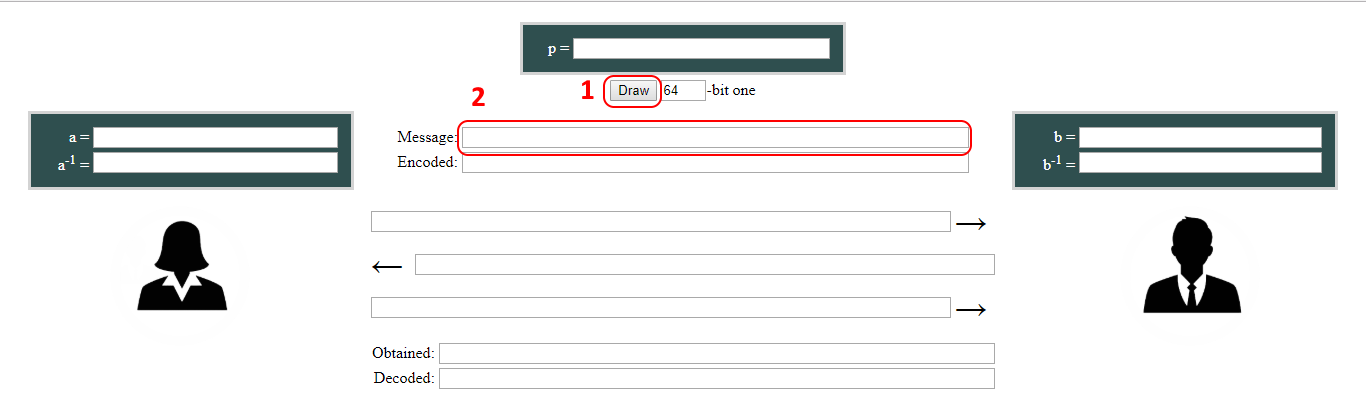
\includegraphics[width=7cm]{../graphics/screenshot commented.png}

\end{document}
